
\documentclass[border=5pt]{standalone}
\usepackage{amsmath}
\usepackage{pgfplots}
\pgfplotsset{compat=1.18}
\usepgfplotslibrary{fillbetween}
\begin{document}
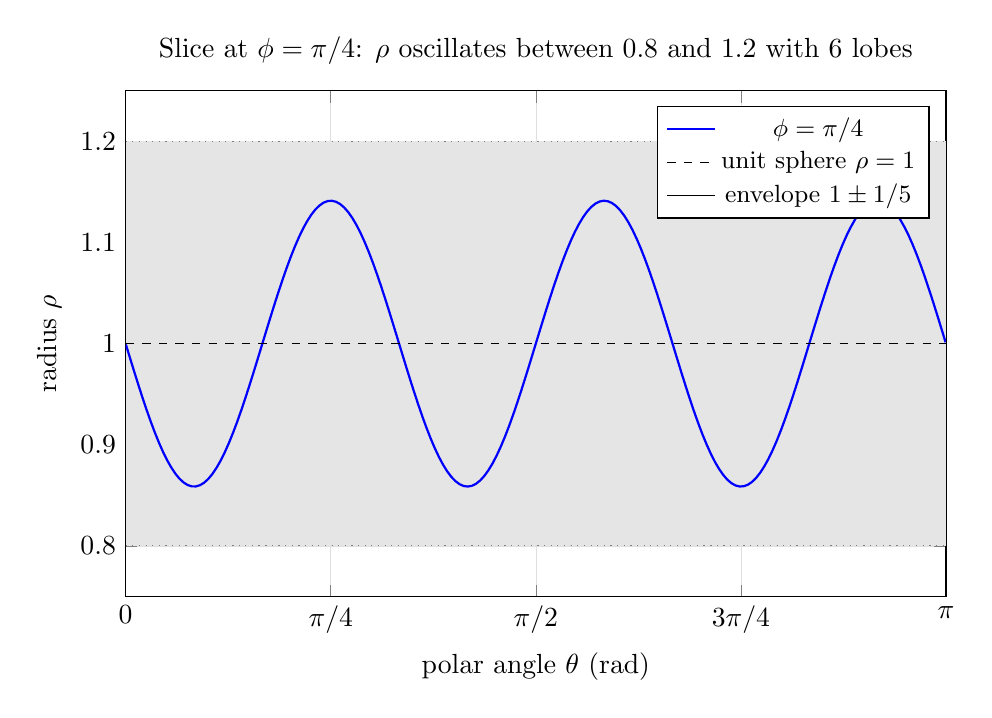
\begin{tikzpicture}
\begin{axis}[
    title={Slice at $\phi=\pi/4$: $\rho$ oscillates between $0.8$ and $1.2$ with 6 lobes},
    width=12cm, height=8cm,
    xlabel={polar angle $\theta$ (rad)},
    ylabel={radius $\rho$},
    xmin=0, xmax=3.1416, ymin=0.75, ymax=1.25,
    xtick={0,0.7854,1.5708,2.3562,3.1416},
    xticklabels={$0$,$\pi/4$,$\pi/2$,$3\pi/4$,$\pi$},
    ytick={0.8,0.9,1.0,1.1,1.2},
    grid=major, grid style={very thin, gray!25},
    legend style={at={(0.98,0.97)}, anchor=north east, font=\small},
    trig format plots=rad,
]
% Slice at phi = pi/4  (sin(5*pi/4) = -1, so radius is 1 - (1/5) sin(6*theta))
\addplot[blue, thick, samples=200, domain=0.001:3.14]
    {1 + 0.2*sin(6*x)*sin(5*pi/4)};
\addlegendentry{$\phi=\pi/4$}

% Reference line at rho = 1 (unit sphere)
\addplot[black, dashed, domain=0:3.1416, samples=2] {1};
\addlegendentry{unit sphere $\rho=1$}

% Filled envelope between 0.8 and 1.2
\addplot[name path=A, draw=none, domain=0:3.1416, samples=2] {0.8};
\addplot[name path=B, draw=none, domain=0:3.1416, samples=2] {1.2};
\addplot[gray!20] fill between[of=A and B];
\addlegendentry{envelope $1\pm 1/5$}

% Dotted envelope curves
\addplot[gray, dotted, domain=0:3.1416, samples=200] {0.8};
\addplot[gray, dotted, domain=0:3.1416, samples=200] {1.2};
\end{axis}
\end{tikzpicture}
\end{document}
